\begin{frame}{von Kármán vortex street}
    The \textit{von Kármán vortex street} phenomenon is a classic example of pattern formation in flows behind bodies, characterized by alternating vortices. 

    \begin{figure}
        \centering
        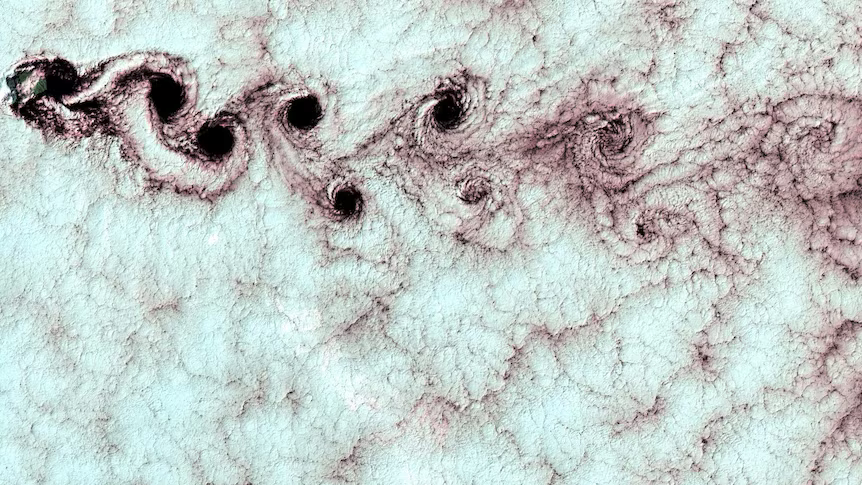
\includegraphics[width=0.6\linewidth]{graphics/example_atmos.png}
        \caption{Atmospheric von Kármán vortex street, showcasing swirling vortices caused by airflow around a mountain (taken from \autocite{wiki})}
        \label{fig:example_vortices}
    \end{figure}
\end{frame}

\begin{frame}{Importance and Objectives}
    \textbf{Why It Matters:}
    \begin{itemize}
        \item Simple phenomenon to study complex flow patterns.
        \item Relevant for cloud formations, and leads to vibrations.
        \item Fundamental example in shape optimization and surface coatings.
    \end{itemize}
    
    \textbf{Project Goals:}
    \begin{itemize}
        \item Simulating von Kármán vortex street in 2D flow using Chorin's method.
        \item Analyzing flow patterns, optimizing for various shapes and configurations.
    \end{itemize}
\end{frame}


